% $Id$

\chapter{Plotting examples}

At present, we shall just show some examples.  Detailed explanations of the
examples will occur at some time in the future.

For the most up to date examples and information, the user is directed to
the \pyvisi web site:
\htmladdnormallink{http://pyvisi.sourceforge.net}{http://pyvisi.sourceforge.net}.

\section{plotExample.py}

\begin{pythonCode}
import sys
sys.path.append('../')

# what plotting method are we using?
method = 'pyvisi'

# set up some data to plot
from Numeric import *

x = arange(10, typecode=Float)
y = x**2

# example code for how a user would write a script in pyvisi
from pyvisi import *          # base level visualisation stuff
#from pyvisi.utils import *   # pyvisi specific utils
# import the objects to render the scene using the specific renderer
#from pyvisi.renderers.gnuplot import *   # gnuplot
from pyvisi.renderers.vtk import *       # vtk
   
# define the scene object
# a Scene is a container for all of the kinds of things you want to put 
# into your plot for instance, images, meshes, arrow/vector/quiver plots, 
# contour plots, spheres etc.
scene = Scene()
    
# create a LinePlot object
plot = LinePlot(scene)
    
# add some helpful info to the plot
plot.title = 'Example 2D plot'
plot.xlabel = 'x'
plot.ylabel = 'x^2'

plot.linestyle = 'lines'
    
# assign some data to the plot
plot.setData(x,y)
plot.render()  # need to tell some renderers to finish up stuff here

# render the scene to screen
scene.render(pause=True,interactive=True)

# save the scene out to file
scene.save(fname="plotExample.png", format=PngImage())
scene.save(fname="plotExample.ps", format=PsImage())
\end{pythonCode}

\ifpdf
\begin{figure}
\centerline{%
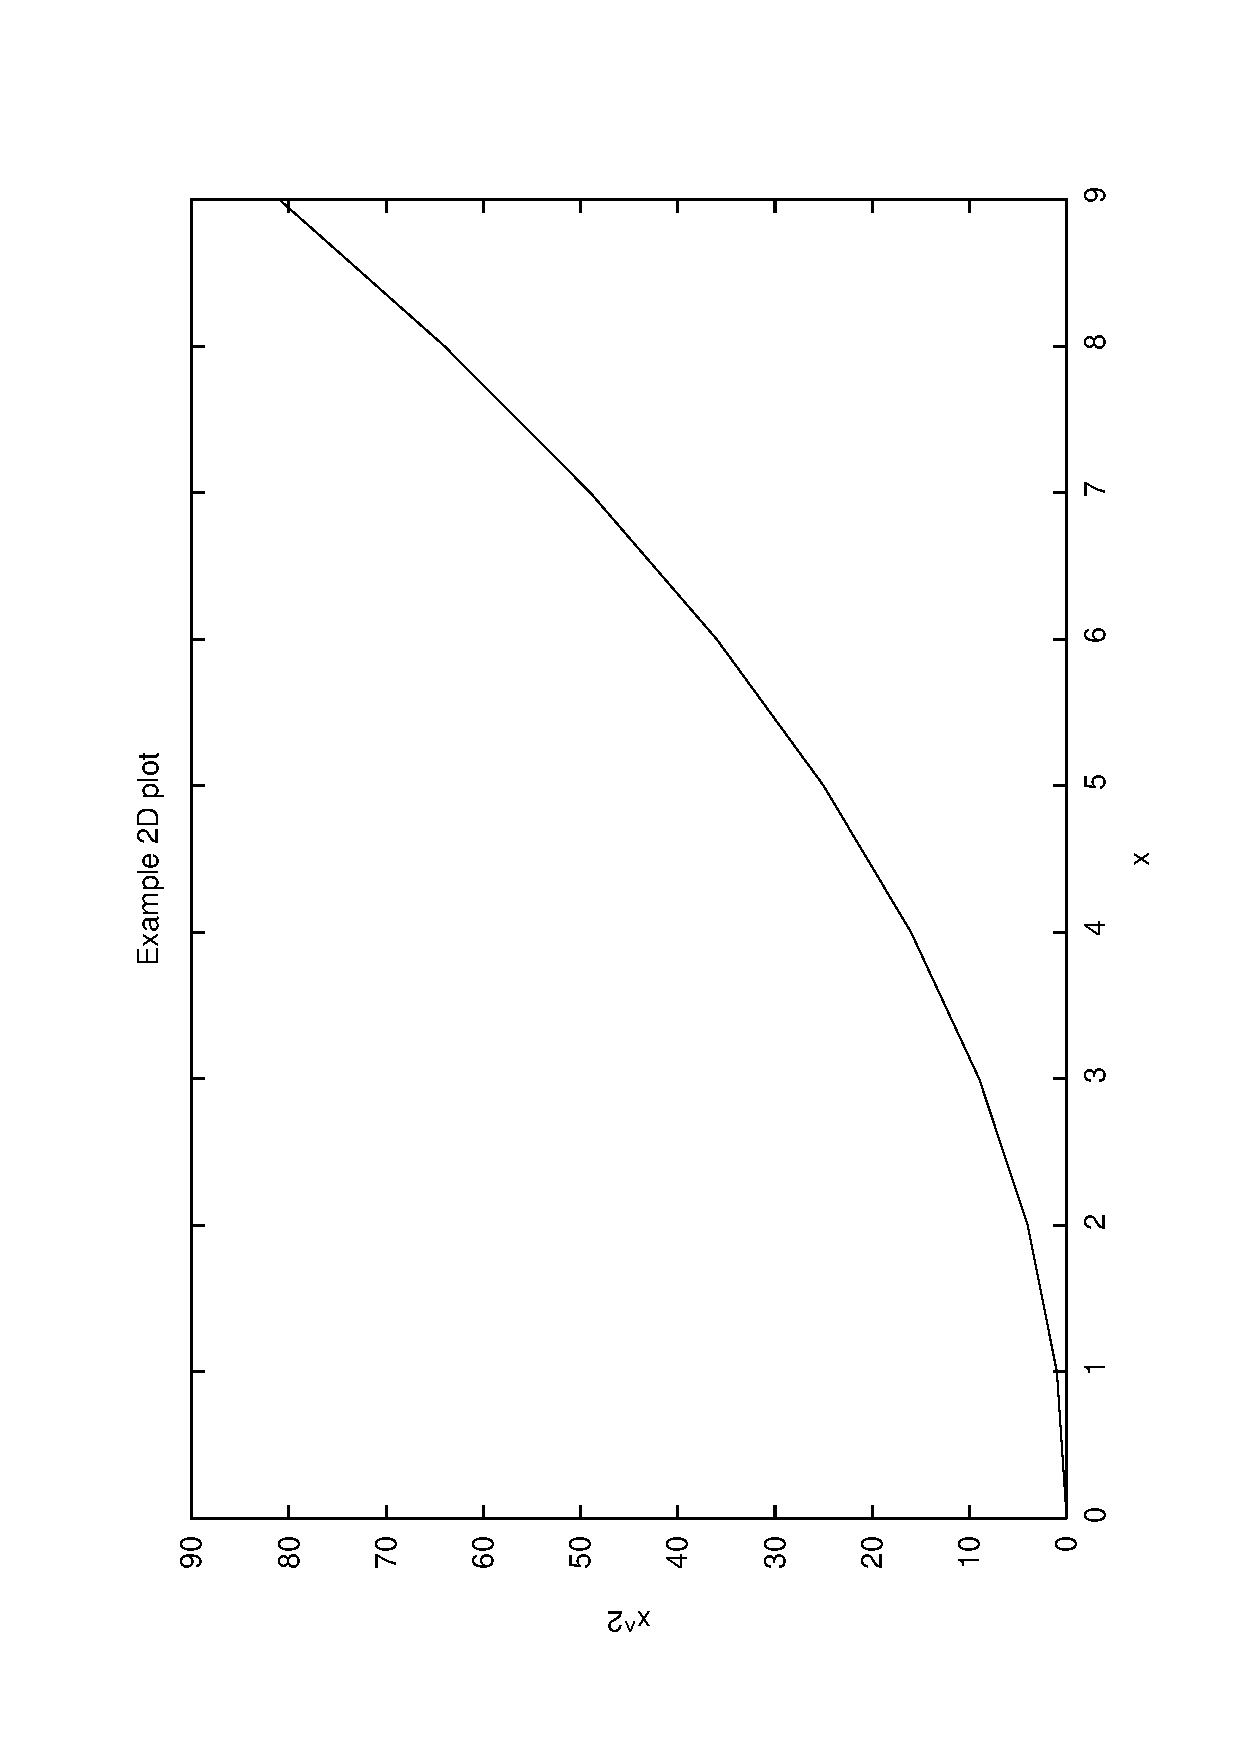
\includegraphics[width=\figwidth]{figures/plotExampleGnuplot}%
}
\caption{Output from gnuplot.}
\end{figure}
\else
\begin{figure}
\centerline{%
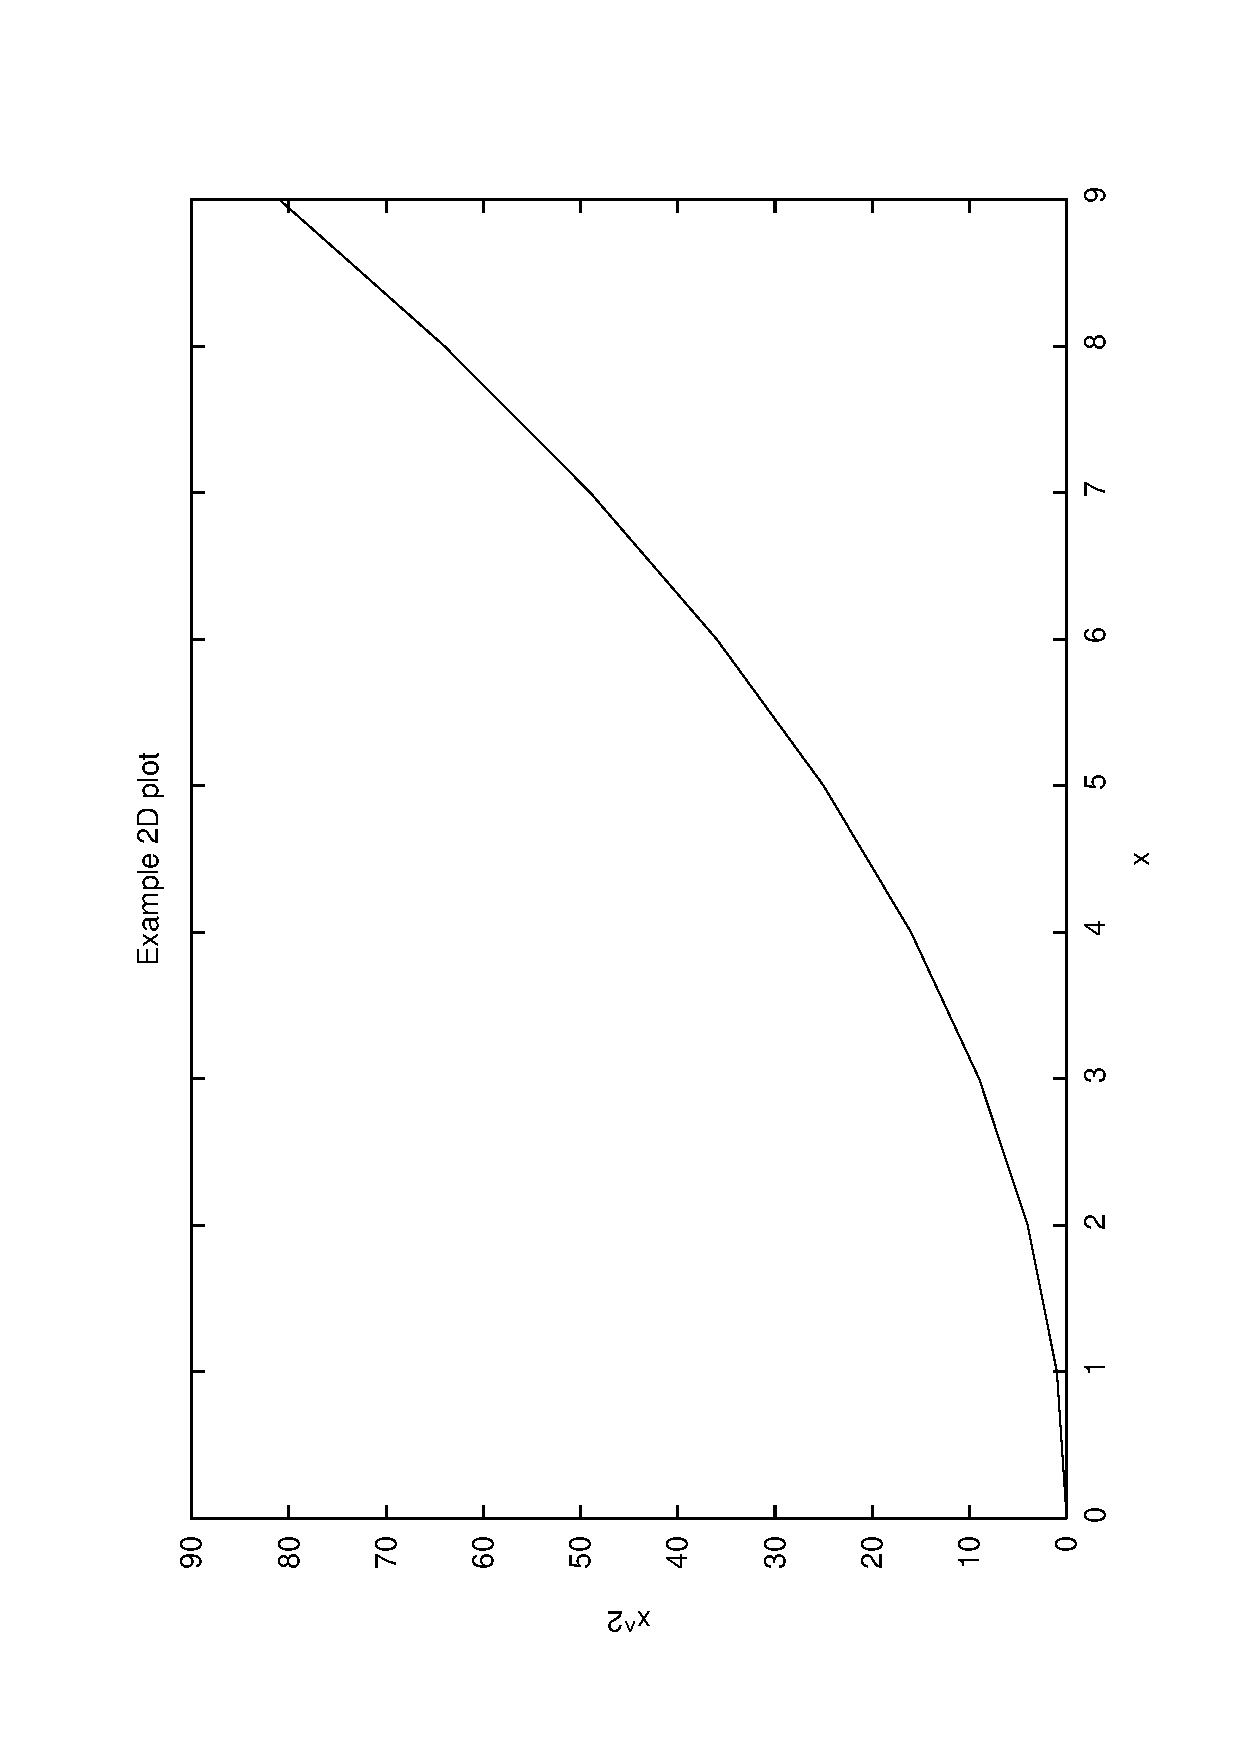
\includegraphics[width=\figwidth,angle=-90]{figures/plotExampleGnuplot}%
}
\caption{Output from gnuplot.}
\end{figure}
\fi

\begin{figure}
\centerline{%
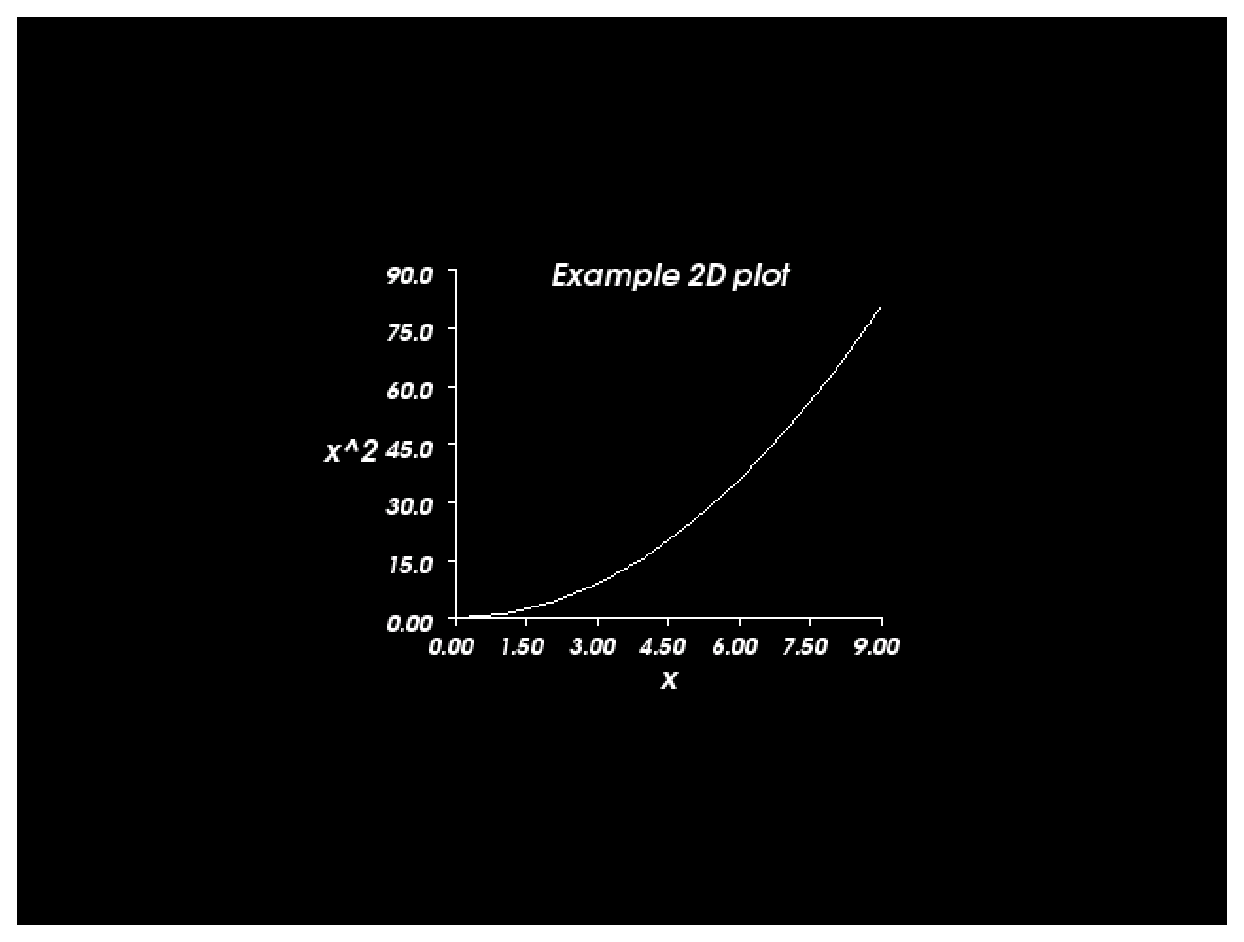
\includegraphics[width=\figwidth]{figures/plotExampleVTK}%
}
\caption{Output from vtk.}
\end{figure}

